\newpage
\maketitle
\begin{center}
\Large \textbf{第301章 MAML算法} \quad 
\end{center}
\begin{abstract}
在本章中,我们将讲解MAML算法的基本原理,并且以Omniglot数据集为例,讲解一个5-way 1-shot的算法实现,并且复现论文中的结果。
\end{abstract}
\section{MAML算法}
在元学习中,最著名的算法当属MAML算法,在本章中,我们将讲解MAML算法数学原理和PyTorch实现技术。
\subsection{Omniglot数据集}
Omniglot数据集的目录结构如下所示:
\begin{figure}[H]
	\caption{Omniglot数据集目录结构}
	\label{f000116}
	\centering
	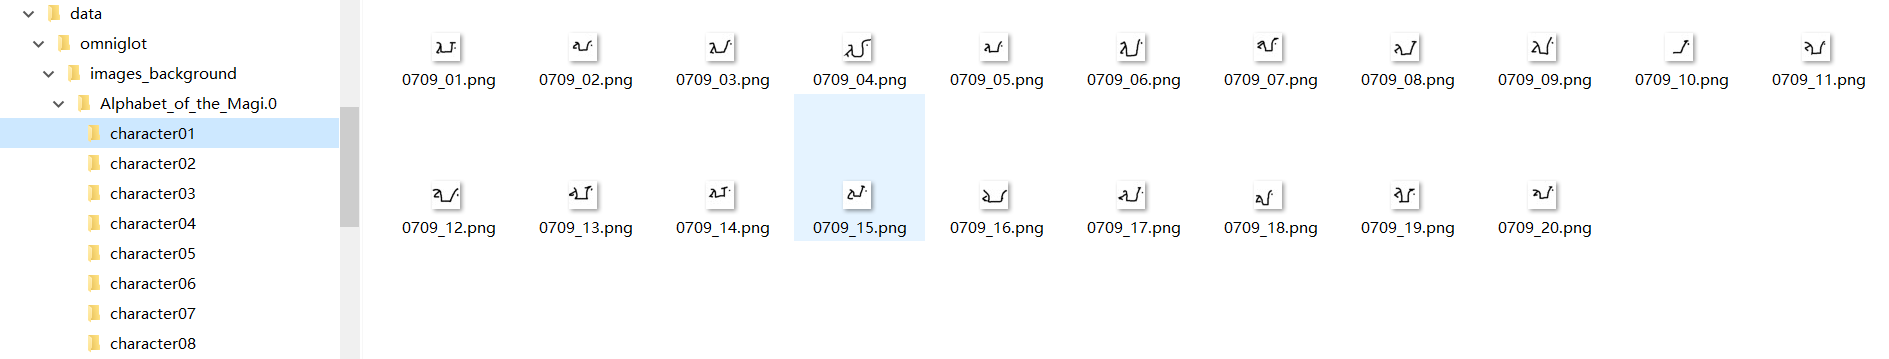
\includegraphics[width=15cm]{images/f000116}
\end{figure}
数据集类代码如下所示:
\lstset{language=PYTHON, caption={Omniglot数据集类}, label={c0301-omniglot-ds}}
\begin{lstlisting}
class OmniglotDs(Dataset):
    def __init__(self, data_dir, k_way, q_query):
        self.file_list = [f for f in glob.glob(data_dir + 
                    '**/character*', recursive=True)]
        self.transform = transforms.Compose([transforms.ToTensor()])
        self.n = k_way + q_query

    def __getitem__(self, idx):
        sample = np.arange(20)
        np.random.shuffle(sample)
        img_path = self.file_list[idx]
        img_list = [f for f in glob.glob(img_path + "**/*.png", 
                    recursive=True)]
        img_list.sort()
        imgs = [self.transform(Image.open(img_file))
                     for img_file in img_list]
        imgs = torch.stack(imgs)[sample[:self.n]]
        return imgs

    def __len__(self):
        return len(self.file_list)   
\end{lstlisting}
代码解读如下所示:
\begin{itemize}
\item 第3、4行:取出图片文件最后一层文件目录的列表,如下所示:
\lstset{language=BASH, caption={self.file\_list内容}, label={c0301-omniglot-ds-file-list}}
\begin{lstlisting}
./data/Omniglot/images_background\Alphabet_of_the_Magi.0\character01
./data/Omniglot/images_background\Alphabet_of_the_Magi.0\character02
./data/Omniglot/images_background\Alphabet_of_the_Magi.0\character03
./data/Omniglot/images_background\Alphabet_of_the_Magi.0\character04
./data/Omniglot/images_background\Alphabet_of_the_Magi.0\character05
./data/Omniglot/images_background\Alphabet_of_the_Magi.0\character06
./data/Omniglot/images_background\Alphabet_of_the_Magi.0\character07
./data/Omniglot/images_background\Alphabet_of_the_Magi.0\character08
\end{lstlisting}
\item 第6行:每个批次中Support Set的大小为k\_way,Query Set的大小为q\_query,该批次的总大小为self.n;
\item 第11行:取到某一个包含图片文件的目录;
\item 第12$\sim$14行取出该目录下所有图片文件列表,每个目录下有20个文件;
\item 第15、16行:类型为list[tensor],将目录下每个图片内容读出来转为tensor,形状为$[1, 28, 28]$,即黑白图片(通道数),分辨率为$28 \times 28$,20个图片文件形成的tensor组成一个list;
\item 第17行:因为在第9行,生成[0,1,...,19]的列表,然后将其随机进行排序,运行结果如下所示:
\lstset{language=BASH, caption={运行原理}, label={c0301-omniglot-ds-get-item}}
\begin{lstlisting}
sample: [ 7  0 18 16 15 17  9 12 11  1  5 14  4  6  8  3  2 10 19 13];
sample[:self.n]: [7 0];
[sample[:self.n]]: [array([7, 0])];
imgs: torch.Size([2, 1, 28, 28]);
\end{lstlisting}
由此可见其形成的是一个训练中用到的迷你批次。
\end{itemize}



